\documentclass{article}
\usepackage[dutch]{babel}
\usepackage[dvipsnames]{xcolor}
\usepackage{tikz}
\usetikzlibrary{chains, scopes, shapes.misc}

% --- Zelfde stijlen als eerst, geen gedoe ---
\tikzset{
  % De basisinstellingen voor de ketting
  nonet/.style={%
    very thick,
    draw,
    align=center,
    rounded corners,
    inner sep=6pt,
    on chain,           % Zegt: "Ik hoor bij de ketting"
    join,               % Zegt: "Trek een pijl naar mij vanaf de vorige"
    every join/.style={->, thick, shorten >=1pt}, % Pijl opmaak
    font=\small
  },
  % Jouw kleurcodes
  tegenpartij/.style={nonet, fill=red!10, draw=red},
  actie/.style={nonet, fill=yellow!20, draw=orange, double, font=\bfseries\small},
  klaar/.style={nonet, fill=green!10, draw=green!50!black, dashed},
  basis/.style={nonet, fill=white, draw=black}
}

\begin{document}

\section*{Dossier: De "Platte" Lijst}

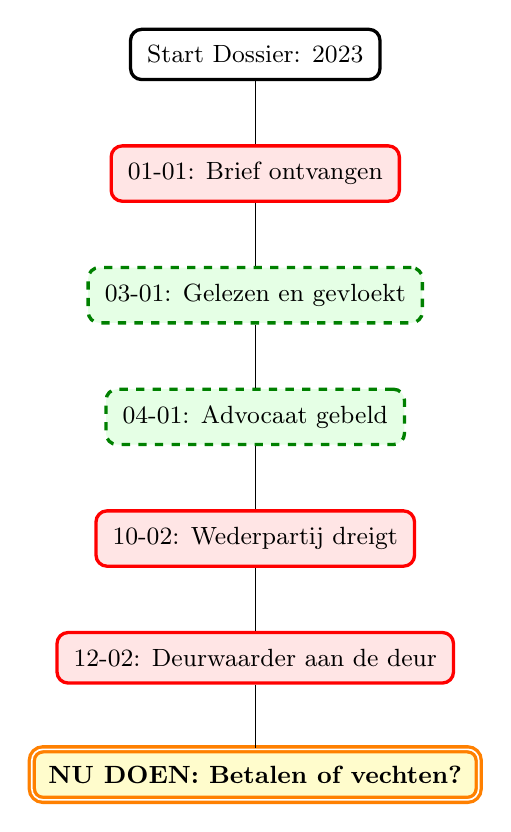
\begin{tikzpicture}[
  start chain=going below,    % Alles wat je toevoegt komt ONDER de vorige
  node distance=8mm           % Afstand tussen de blokjes
  ]

  % --- HIER BEGINT JE LIJST (Geen inspringing nodig!) ---
  
  \node [basis]       {Start Dossier: 2023};
  
  \node [tegenpartij] {01-01: Brief ontvangen};
  
  \node [klaar]       {03-01: Gelezen en gevloekt};
  
  \node [klaar]       {04-01: Advocaat gebeld};
  
  \node [tegenpartij] {10-02: Wederpartij dreigt};
  
  \node [tegenpartij] {12-02: Deurwaarder aan de deur};
  
  \node [actie]       {NU DOEN: Betalen of vechten?};

  % --- EINDE LIJST ---

\end{tikzpicture}

\end{document}